\section{Design}
\label{sec:architecture}

\subsection{System Architecture}

KV-Direct enables \textit{remote direct key-value access}.
Clients send \textit{KV-Direct operations} (\S\ref{sec:kv-operations}) to KVS server while the \ournic{} processes the requests and sending back results, bypassing the CPU.
-The \ournic{} on KVS server is an FPGA reconfigured as a \textit{KV processor} (\S\ref{sec:kv-processor}).
Figure~\ref{fig:kvdirect-arch} shows the architecture of KV-Direct.

\subsection{KV-Direct Operations}
\label{sec:kv-operations}

\begin{table}
\centering
\caption{KV-Direct operations.}
\label{tab:kv-operations}
\small
\begin{tabular}{p{.16\textwidth}|p{.28\textwidth} }
\toprule
get ($k$) $\rightarrow v$ & Get the value of key $k$. \\
\midrule
put ($k, v$) $\rightarrow$ bool & Insert or replace a $(k, v)$ pair. \\
\midrule
delete ($k$) $\rightarrow$ bool & Delete key $k$. \\
\midrule
\midrule
update{\_}scalar2scalar ($k, \Delta, \lambda(v, \Delta) \rightarrow v$) $\rightarrow v$ & Atomically update the value of key~$k$ using function~$\lambda$ on scalar~$\Delta$, and return the original value. \\
\midrule
update{\_}scalar2vector ($k, \Delta, \lambda(v, \Delta) \rightarrow v$) $\rightarrow [v]$ & Atomically update all elements in vector~$k$ using function~$\lambda$ and scalar~$\Delta$, and return the original vector. \\
\midrule
update{\_}vector2vector ($k, [\Delta], \lambda(v, \Delta) \rightarrow v$) $\rightarrow [v]$ & Atomically update each element in vector~$k$ using function~$\lambda$ on the corresponding element in vector~$[\Delta]$, and return the original vector. \\
\midrule
reduce ($k, \Sigma, \lambda(v, \Sigma) \rightarrow \Sigma$) $\rightarrow \Sigma$ & Reduce vector~$k$ to a scalar using function~$\lambda$ on initial value, and return the reduction result~$\Sigma$. \\
\midrule
filter ($k, \lambda(v) \rightarrow$ bool) $\rightarrow [v]$ & Filter elements in a vector~$k$ by function~$\lambda$, and return the filtered vector. \\
\bottomrule
\end{tabular}
\vspace{-10pt}
\end{table}

KV-Direct extends one-sided RDMA operations to key-value operations, as summarized in Table~\ref{tab:kv-operations}.
In addition to standard KVS operations as shown in the top part of Table~\ref{tab:kv-operations}, KV-Direct supports vector operations, as well as \textit{active messages}~\cite{eicken1992active} as a generalization to atomic operations.
Active messages enable near-memory computation and save communication and synchronization cost.

When a vector operation update, reduce or filter is operated on a key, its value is treated as an array of fixed-bit-width elements.
Each function $\lambda$ operates on one element in the vector, a client-specified parameter~$\Delta$, and/or an initial value~$\Sigma$ for reduction.
For efficiency, the $\lambda$ functions are compiled into hardware logic, so they need to be pre-registered by the KVS client and substituted with numeric opcodes during runtime.
The KV-Direct development toolchain duplicates the $\lambda$ several times to leverage parallelism in FPGA and match computation throughput with PCIe throughput, then compiles it into hardware logic using an high-level synthesis (HLS) tool~\cite{aoc}.
The HLS tool automatically extracts data dependencies in the duplicated function and generates a fully pipelined programmable logic.
%Before executing the KVS client, the programmable NIC on KVS servers should be loaded with the hardware logic containing the unrolled $\lambda$.

Update operations with active messages not only cover standard scalar atomic operations such as compare-and-swap and fetch-and-add, but also capable of general stream processing on a vector value.
For example, a network processing application may interpret the vector as a stream of packets for network functions~\cite{li2016clicknp} or a bunch of states for packet transactions~\cite{sivaraman2016packet}.
Single-object transaction processing completely in the programmable NIC is also possible, \eg, wrapping around S\_QUANTITY in TPC-C benchmark~\cite{council2010tpc}.
Vector reduce operation supports neighbor weight accumulation in PageRank~\cite{page1999pagerank}.
Non-zero values in a sparse vector can be fetched efficiently with vector filter operation.

\subsection{KV Processor}
\label{sec:kv-processor}

\begin{figure}[t]
\centering
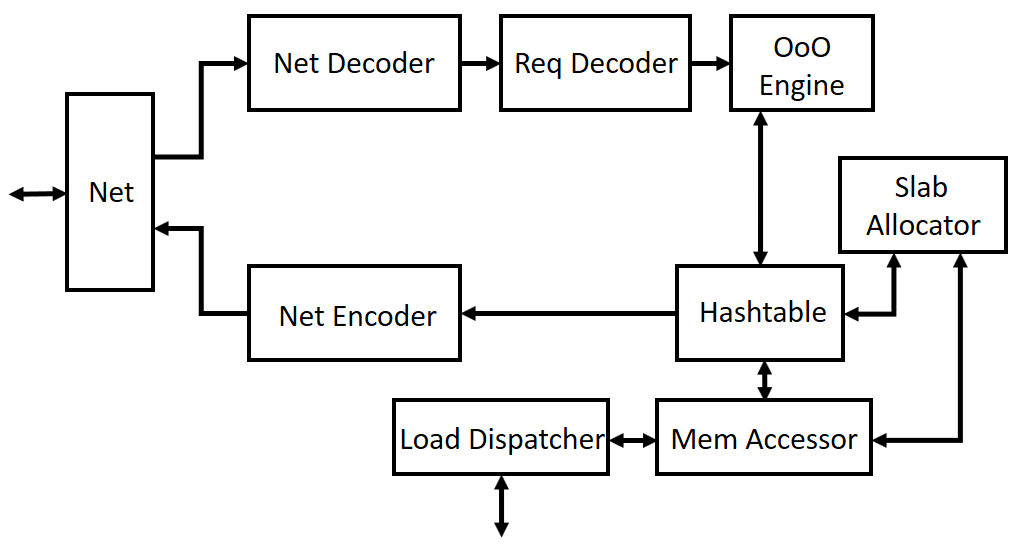
\includegraphics[width=0.4\textwidth,page=1]{processor_architecture.PNG}
\caption{KV processor architecture.}
\label{fig:kvprocessor-arch}
\vspace{-10pt}
\end{figure}

As shown in Figure~\ref{fig:kvprocessor-arch}, the KV processor receives packets from the on-board NIC, decodes vector operations and buffers KV operations in the reservation station (\S\ref{sec:ooo}).
Next, the out-of-order engine (\S\ref{sec:ooo}) issues independent KV operations from reservation station into the operation decoder.
Depending on the operation type, the KV processor looks up the hash table (\S\ref{sec:hashtable}) and executes the corresponding operations.
To minimize the number of memory accesses, small KV pairs are stored \textit{inline} in the hash table, others are stored in dynamically allocated memory from the slab memory allocator (\S\ref{sec:slab}).
Both the hash index and the slab-allocated memory are managed by a unified memory access engine (\S\ref{sec:dram-cache}), which accesses the host memory via PCIe DMA and caches a portion of host memory in on-board DRAM.
After the KV operation completes, the result is sent back to the out-of-order execution engine (\S\ref{sec:ooo}) to find and execute matching KV operations in reservation station.

As discussed in \S\ref{sec:challenge}, the scarcity of PCIe operation throughput requires the KV processor to be frugal on DMA accesses.
For GET operation, at least one memory read is required.
For PUT or DELETE operation, one read and one write are minimal.
KV-Direct carefully designs the hash table to achieve close to ideal DMA accesses per lookup and insertion, as well as the memory allocator to achieve $<$~0.1 amortized DMA operations per dynamic memory allocation.

\subsubsection{Hash Table}
\label{sec:hashtable}

\begin{figure}[t]
\centering
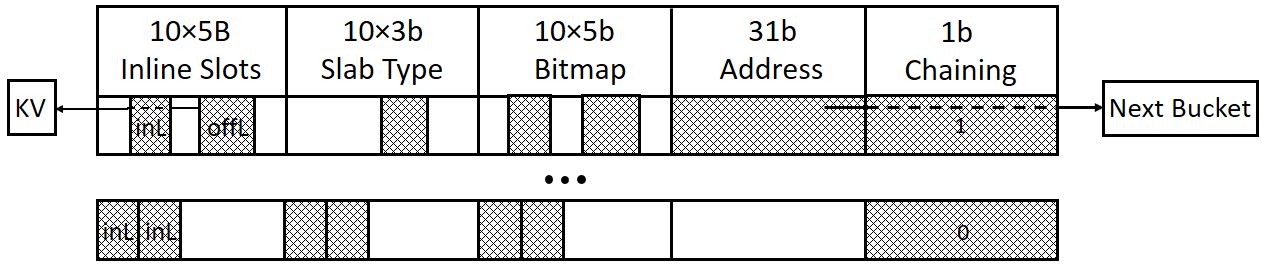
\includegraphics[width=.5\textwidth,page=1]{hashline.PNG}
\caption{Hash index structure. Each line is a hash bucket containing 10 hash slots, 3 bits of slab memory type per hash slot, one bitmap marking the beginning and end of inline KV pairs and a pointer to the next chained bucket on hash collision.}
\label{fig:hashtable}
\vspace{-10pt}
\end{figure}

To store variable-sized KVs, the KV storage is partitioned into two parts. The first part is a hash index (Figure~\ref{fig:hashtable}), which consists a fixed number of \textit{hash buckets}. Each hash bucket contains several \textit{hash slots} and some metadata. The rest of the memory is dynamically allocated, and managed by a slab allocator (\S\ref{sec:slab}).
A \textit{hash index ratio} configured at initialization time determines the percentage of the memory allocated for hash index.
The choice of hash index ratio will be discussed in \S\ref{sec:hashtable-eval}.

%\textbf{Hash Table.}
%Each bucket includes 10 hash slots, 3b type code per slot, 50b metadata, plus 31b address and a valid bit of the next chained bucket, as shown in Figure~\ref{fig:hashtable}.
%For offline KVs, each hash slot needs to store 31b of address, 9b of secondary hash and 3b type code for the slab size.
%For inline KVs, to mark the begin and end of each hash slot, as well as the separation between inline key and value, the information is encoded in a 50b metadata corresponding to 50 bytes of hash slots.
%The inline keys and secondary hashes of offline keys in all hash slots are compared in parallel, and the first match is found.

Each hash slot includes a pointer to the KV data in dynamically allocated memory and a secondary hash for quick probabilistic comparison.
Assuming a 64~GiB KV storage in host memory and 32-byte allocation granularity, the pointer requires 31 bits.
A secondary hash of 9 bits gives a 1/512 false positive possibility.
Cumulatively, the hash slot size is 5 bytes.
To determine the hash bucket size, we need to trade-off between the number of hash slots per bucket and the DMA throughput.
Figure~\ref{fig:dma-tput} shows that the DMA read throughput below 64B granularity is bound by PCIe latency and parallelism in the DMA engine.
A bucket size less than 64B is suboptimal due to increased possibility of hash collision.
On the other hand, increasing the bucket size above 64B would decrease hash lookup throughput.
So we choose the bucket size to be 64 bytes.

\begin{figure}[t]
\centering
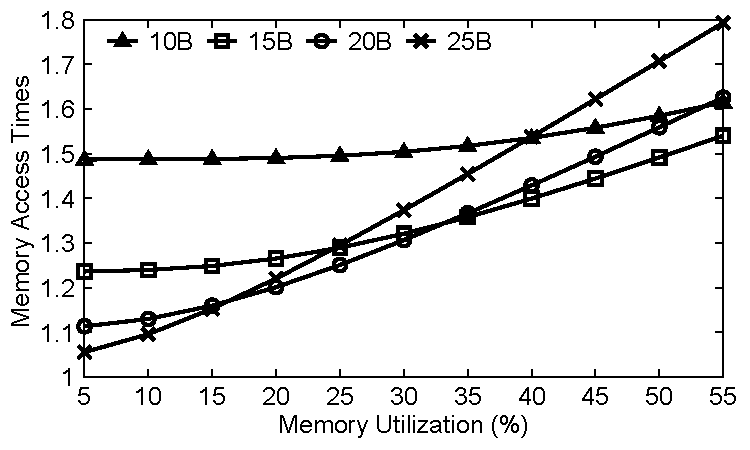
\includegraphics[width=0.33\textwidth]{inline_thresh.pdf}
\caption{Average memory access count under varying inline thresholds (10B, 15B, 20B, 25B) and memory utilizations.}
\label{fig:inline-offline}
\vspace{-10pt}
\end{figure}

Small KVs are stored \textit{inline} in the hash index to save the additional memory access to fetch KV data.
An inline KV may span multiple hash slots.
It might not be optimal to inline all KV that can fit in a bucket.
To minimize average access time, assuming that smaller and larger keys are equally likely to be accessed, it is more desirable to inline KVs smaller than an \textit{inline threshold}.
As shown in Figure~\ref{fig:inline-offline}, for a certain inline threshold, the average memory access count increases with memory utilization, due to more hash collisions.
Higher inline threshold shows a more steep growth curve of memory access count, so an optimal inline threshold can be found to minimize memory accesses under a given memory utilization.
As with hash index ratio, the inline threshold can also be configured at initialization time.

When all slots in a bucket are filled up, there are several solutions to resolve hash collisions.
Cuckoo hashing~\cite{pagh2004cuckoo} and hopscotch hashing~\cite{herlihy2008hopscotch} achieve constant-time lookup by moving occupied slots during insertion.
In write-intensive workload, the memory access time under high load factor would experience large fluctuations.
Linear probing may suffer from primary clustering, therefore its performance is sensitive to the uniformity of hash function.
We choose \textit{chaining} to resolve hash conflicts, which balances lookup and insertion, while being more robust to hash clustering.


%In KV-Direct, we measure memory utilization instead of load factor, because chaining has dynamic size and that we care more about the overall storage efficiency counting all indexing, metadata and memory fragmentation overhead.
%Clearly, small KVs cause lower memory utilization due to metadata overhead.
%The optimal hash index ratio is chosen at initialization time according to workload to balance average access time and memory utilization.

\subsubsection{Slab Memory Allocator}
\label{sec:slab}

Chained hash slots and non-inline KVs need dynamic memory allocation.
We choose slab memory allocator~\cite{bonwick1994slab} to achieve $O(1)$ average memory access per allocation and deallocation. The main slab allocator logic runs on host CPU and communicates with the KV-processor through PCIe.
Slab allocator rounds up allocation size to the nearest power of two, called \textit{slab size}.
It maintains a \textit{free slab pool} for each possible slab size (32, 64, \ldots, 512 bytes), and a global \textit{allocation bitmap} to help to merge small free slabs back to larger slabs.
Each free slab pool is an array of \textit{slab entries} consisting of an address field and a slab type field indicating the size of the slab entry.
The free slab pool can be cached on the NIC. The cache syncs with the host memory in batches of slab entries. Amortized by batching, less than 0.07 DMA operation is needed per allocation or deallocation.
When a small slab pool is almost empty, larger slabs need to be split.
Because the slab type is already included in a slab entry, in \textit{slab splitting}, slab entries are simply copied from the larger pool to the smaller pool, without the need for computation.
Including slab type in the slab entry also saves communication cost because one slab entry may contain multiple slots.

On deallocation, the slab allocator needs to check whether the freed slab can be merged with its neighbor, requiring at least one read and write to the allocation bitmap.
Inspired by garbage collection, we propose \textit{lazy slab merging} to merge free slabs in batch when a slab pool is almost empty and no larger slab pools have enough slabs to split.

\subsubsection{Out-of-Order Execution Engine}
\label{sec:ooo}
%
%\begin{figure}[t]
%\centering
%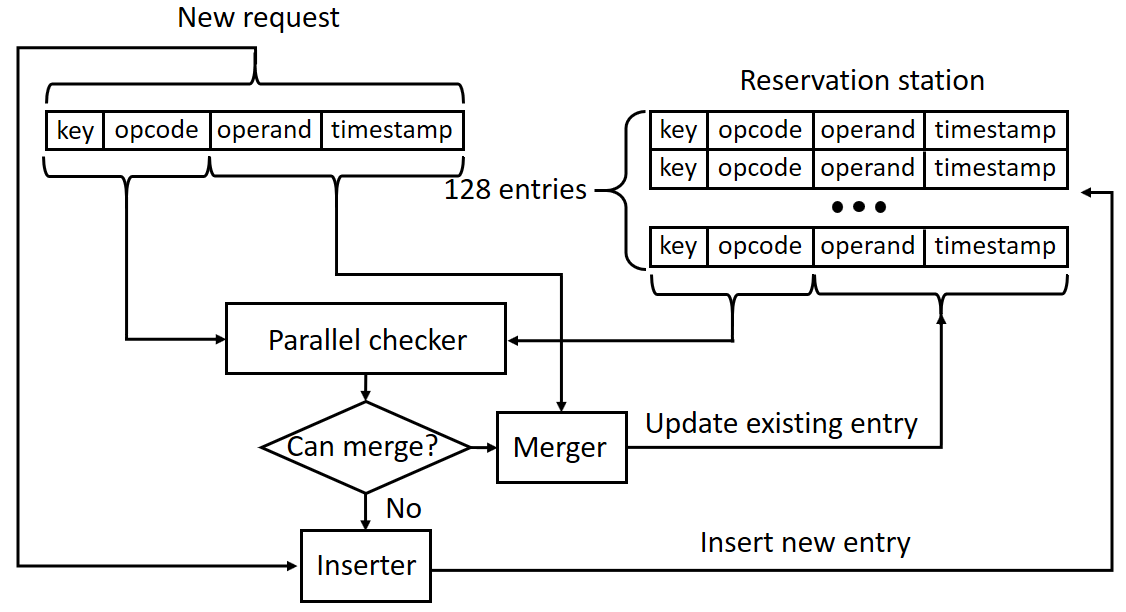
\includegraphics[width=.45\textwidth,page=1]{dynamic_scheduler.PNG}
%\caption{Dynamic operation scheduler.}
%\label{fig:ooo-mem-access}
%\vspace{-10pt}
%\end{figure}

Dependency between two KV operations with the same key in the KV processor will lead to data hazard and pipeline stall.
This problem is magnified in single-key atomics where all operations are dependent, thus limiting the atomics throughput.
We borrow the concept of dynamic scheduling from computer architecture and implement a \textit{reservation station} to track all in-flight KV operations and their \textit{execution context}.
To saturate PCIe, DRAM and the processing pipeline, up to 256 in-flight KV operations are needed.
However, comparing 256 16-byte keys in parallel would take 40\% logic resource of our FPGA.
Instead, we store the KV operations in a small hash table in on-chip RAM, indexed by the hash of the key.
To simplify hash collision resolution, we regard KV operations with the same hash as dependent, so there may be false positives, but it will never miss a dependency.
Operations with the same hash are organized in a chain and examined sequentially.
Hash collision would degrade the efficiency of chain examination, so the reservation station contains 1024 hash slots to make hash collision possibility below 25\%.

The reservation station not only holds pending operations, but also caches their latest values for \textit{data forwarding}.
When a KV operation is completed by the main processing pipeline, its result is returned to the client, and the latest value is forwarded to the reservation station.
Pending operations in the same hash slot are checked one by one, and operations with matching key are executed immediately and removed from the reservation station.
For atomic operations, the computation is performed in a dedicated execution engine.
For write operations, the cached value is updated.
The execution result is returned to the client directly.
After scanning through the chain of dependent operations, if the cached value is updated, a PUT operation is issued to the main processing pipeline for cache write back.
This data forwarding and fast execution path enable single-key atomics to be processed one operation per clock cycle (180~Mops), eliminate head-of-line blocking under workload with popular keys, and ensure consistency because no two operations on the same key can be in the main processing pipeline simultaneously.


\subsubsection{DRAM Load Dispatcher}
\label{sec:dram-cache}

\begin{figure}[t]
\centering
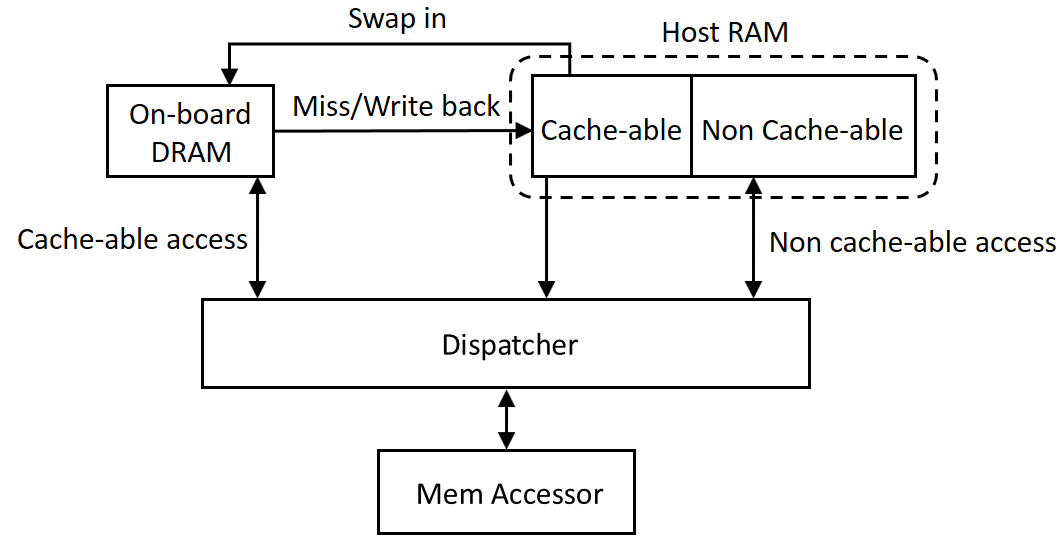
\includegraphics[width=0.4\textwidth,page=1]{load_balancer.PNG}
\caption{DRAM load dispatcher.}
\label{fig:cache}
\vspace{-15pt}
\end{figure}

To further save the burden on PCIe, we dispatch memory accesses between PCIe and the on-board DRAM.
Our on-board DRAM has 4~GiB size and 12.8~GB/s throughput, which is an order of magnitude smaller than the KVS storage on host DRAM (64~GiB) and slightly slower than the PCIe link (14~GB/s).
One approach is to put a fixed portion of the KVS in on-board DRAM. However, the on-board DRAM is too small to carry a significant portion of memory accesses.
The other approach is to use the on-board DRAM as a cache for host memory, the throughput would degrade due to the limited throughput of our on-board DRAM.

We adopt a hybrid solution to use the DRAM as a cache for a fixed portion of the KVS in host memory, as shown in Figure~\ref{fig:cache}.
The portion of cache-able memory in the entire KVS memory is called \textit{load dispatch ratio}.
With a larger load dispatch ratio $l$, more load is dispatched to the on-board DRAM and the cache hit ratio $h(l)$ would increase.
To balance load on PCIe and on-board DRAM, the load dispatch ratio $l$ should be optimized such that:
$$\frac{l}{tput_{DRAM}} = \frac{(1-l) + l \cdot (1-h(l))}{tput_{PCIe}}$$

Specifically, under uniform workload, let $k$ be the ratio of on-board DRAM size and host KV storage size, cache hit ratio $h(l) = k/l$.
Under long-tail workload with Zipf distribution, assume $n$ is the total number of KVs, approximately $h(l) = \frac{\log (kn/l)}{\log n} = \frac{\log kn}{\log n} - \frac{1}{\log n}\log l$.
For these simple key distributions, we can derive a closed form of the optimal load dispatch ratio $l$.



\egg{
\subsubsection{Congestion Avoidance}
\label{sec:congestion-avoidance}

In addition to throughput, another important factor is latency.
From the client's perspective, the KV processor is a path with multiple bottlenecks and buffers, \eg, PCIe and DRAM access.
If all buffers in the KV processor are filled up, the GET latency would exceed 10~$\mu$s.
To mitigate the bufferbloat problem, we implement a congestion avoidance logic to limit the number of in-flight KV operations \textit{inside the KV processor}.
The KV processor maintains a \textit{KV operation window} and leverages credit-based flow control mechanism in RDMA to back-pressure KVS clients.
To adapt KV operation window size to the workload, we measure the running average of KV processing delay and adjust the window size according to TCP Vegas congestion avoidance algorithm~\cite{brakmo1995tcp}.
%We use delay as the congestion signal instead of ECN, because the queues whose sizes are hard to measure.
}
